\setcounter{chapter}{2}
\chapter[\MakeUppercase{Triển khai thuật toán MUSIC trên thiết bị SDR}]{Triển khai thuật toán MUSIC trên thiết bị SDR}
Trong chương này, trước hết trình bày việc triển khai thuật toán MUSIC trên GNU Radio với dữ liệu giả lập từ Matlab để tránh các hạn chế của sóng vô tuyến như: nhiễu đa đường, phản xạ, nhiễu xạ, tán xạ gây khó khăn cho độ chính xác của thuật toán cũng như kiểm tra hoạt động của việc lập trình các khối OTT (Out Of Tree Modules) trên GNU Radio. Sau đó áp dụng trên các thiết bị SDR, phân tích các khó khăn và hướng giải quyết chúng.

\section{Thực thi hệ thống dựa trên GNU Radio và dữ liệu giả lập từ Matlab}
\subsection{Mô tả dữ liệu mô phỏng}
Vẫn áp dụng mô hình tín hiệu như ở mục 1.2: $\mathbf{x}(t) = \mathbf{A}(\Theta)\mathbf{s}(t) + \mathbf{n}(t)$, các thông số mô phỏng như phía dưới:
{\renewcommand\labelitemi{}
\begin{itemize}
	\item $f = 914\textrm{MHz}$		\hspace{1.65cm}\% Tần số
	\item $\lambda = c \div f = 0.328 m$	\hspace{0.47cm}\% Bước sóng
	\item $M = 4$				\hspace{2.88cm}\% Sổ phần tử anten của mảng thu
	\item $d = 0.5 \times \lambda$		\hspace{2.2cm}\% Khoảng cách giữa các phần tử anten mảng thu (\textbf{ULA})
	\item $D = 1$				\hspace{2.92cm}\% Số phần tử nguồn
	\item $angle = 85 \times (\pi \div 180)$ \% Góc tới của tín hiệu
	\item $gain = 0$				\hspace{2.5cm}\% Hệ số khuếch đại
	\item $SNR = 15 dB$			\hspace{1.57cm}\% Tỷ lệ tín hiệu tạp âm
	\item $k = 2 \times \pi \div \lambda$	\hspace{1.56cm}\% Hệ số sóng
	\item $K = 5000$				\hspace{2.3cm}\% Số mẫu thu thập
\end{itemize}
\begin{subequations}
\label{eq:all}
\begin{align}
\label{eq:model_a}
    \mathbf{s} &=
    \begin{bmatrix}
   	20^{\frac{SNR}{10}}\times \mathrm{randn}(1, K) + j \times \mathrm{randn}(1, K)
    \end{bmatrix}\\
\label{eq:model_b}
    \mathbf{A} &=
    \begin{bmatrix}
	10^{\frac{gain}{10}} \times \mathrm{exp}\{j \times k \times (0:M-1) \times d \times \cos(angle)\}
    \end{bmatrix}^T \\
\label{eq:model_c}
 \mathbf{n} &=
    \begin{bmatrix}
	\mathrm{randn}(M, K) + j \times \mathrm{randn}(M, K)
    \end{bmatrix} \\
\label{eq:model_d}
 \mathbf{x} &=
    \begin{bmatrix}
	\mathbf{A}\mathbf{s} + \mathbf{n}
    \end{bmatrix}
%\end{equation} 
\end{align}
\end{subequations}

Sử dụng Matlab tạo mô phỏng dữ liệu đầu vào với những thông số như trên, thu được được ma trận $\mathbf{x}(t) \in \mathbb{C}^{4 \times 5000}$, lưu trữ nó vào file \textit{source.mat} bằng hàm có sẵn của Matlab. Việc tiếp theo là đưa dữ liệu mô phỏng vào GNU Radio, dưới đây là phương pháp tạo khối để nhận vào dữ liệu mô phỏng và khối tính toán, hiển thị DOA cho người dùng.

\subsection{Sơ đồ khối và mô tả sơ đồ khối}

Có nhiều cách để tạo một khối OTT trên GNU Radio, đơn giản nhất là sử dụng ngay Python Block là một khối trong thư viện của GNU Radio, cho phép lập trình một khối mới ngay lập tức với ngôn ngữ Python. Tuy nhiện hạn chế ở hiệu năng và không thể tùy biến được nhiều và sâu cho khối, vì vậy chỉ nên sử dụng khi kiếm tra nhanh thuật toán. Một cách nữa được nhà phát hành cung cấp chính thức cho các lập trình viên đó là công cụ gr\_modtool.

\begin{figure}[!htb]
%\hfill
\subfigure[Khối Python Block trên GNU Radio]{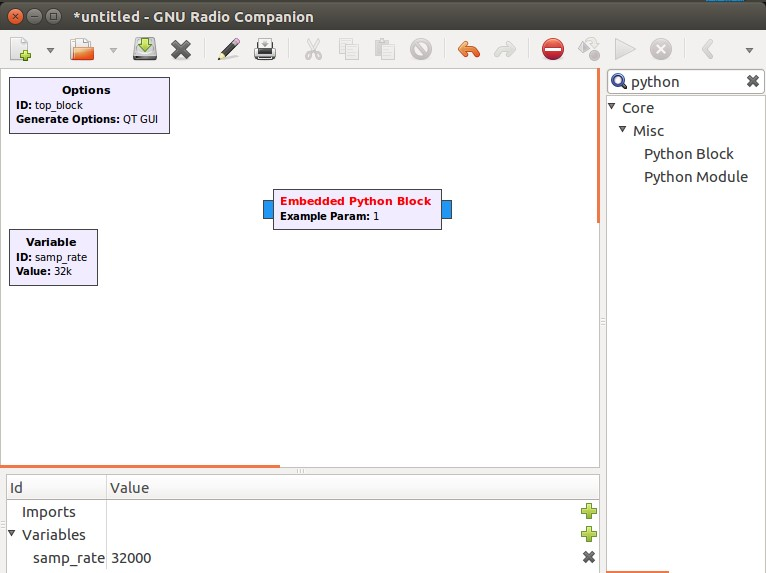
\includegraphics[width=0.49\linewidth]{figures/pythonblock.jpg}}
\hfill
\subfigure[Lập trình cho khối Python Block]{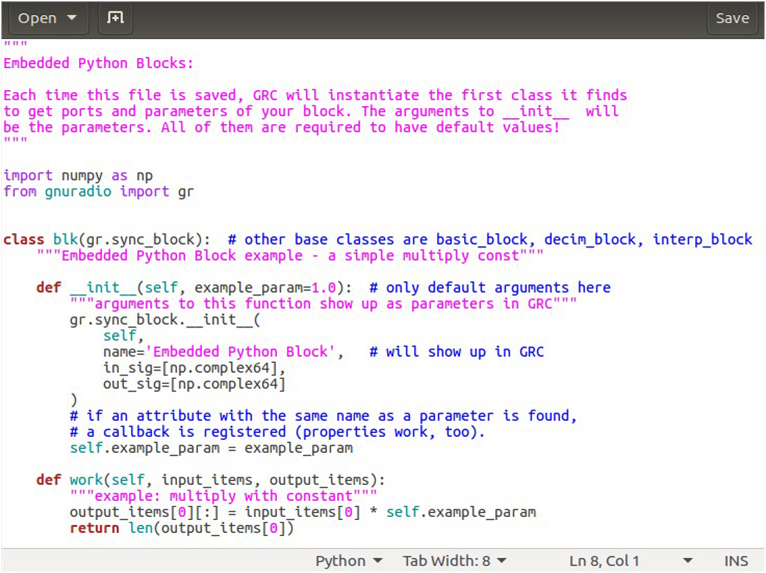
\includegraphics[width=0.49\linewidth]{figures/pythonblock2.jpg}}
\hfill
\caption{Tạo khối với Python Block trên GNU Radio}
\label{fig:pythonblock}
\end{figure}

Công cụ gr\_modtool được tích hợp sẵn vào GNU Radio từ năm 2010, sử dụng để tạo sẵn template các khối OTT với chức năng đa dạng cho người dùng, giúp bỏ qua các bước phải lặp đi lặp lại như: tạo các mã soạn sẵn, sửa makefile, ... Hỗ trợ lập trình khối cho GNU Radio với ngôn ngữ C++ và Python với liên kết bằng SWIG được tích hợp sẵn, việc cài đặt các khối sau khi lập trình được thực  hiện tự động bằng CMAKE, hoàn toàn phù hợp cho cả người mới bắt đầu vào các mục đích nghiên cứu chuyên sâu. Hình \ref{fig:grmodtool} ví dụ một Module được tạo bằng gr\_modtool chứa nhiều thư mục và file đã tạo sẵn, một Module có thể chứa nhiều khối OTT.

\begin{figure} [h]
	\centering
	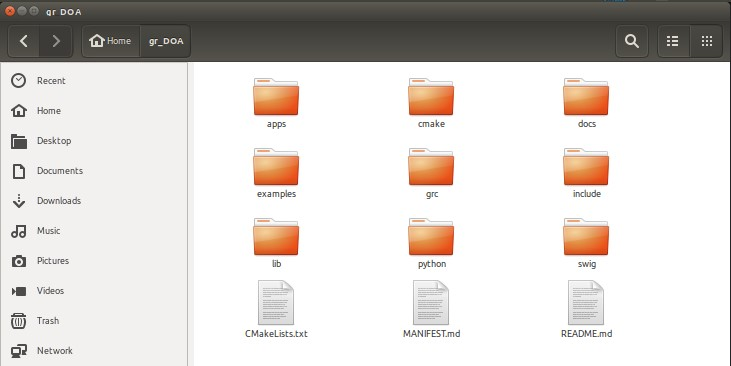
\includegraphics[width=1\linewidth]{figures/grmodtool.jpg}
	\caption{Module được tạo bằng gr\_modtool}
	\label{fig:grmodtool}
\end{figure}

Tiếp theo, cần xác định loại khối cho các mục đích khác nhau, dưới đây là 4 loại khối được GNU Radio cung cấp:
\renewcommand{\labelitemi}{$\bullet$}
\begin{itemize}
	\item Synchronous Blocks: Số mẫu đầu vào và đầu ra của khối là bằng nhau (\textbf{1 / 1}).
	\item Decimation Blocks: Cứ \textbf{N} mẫu đầu vào thì có 1 mẫu đầu ra (\textbf{N / 1}).
	\item Interpolation Blocks: Cứ 1 mẫu đầu vào thì có \textbf{M} mẫu đầu ra (\textbf{1 / M}).
	\item General Blocks: Tùy chỉnh tỷ lệ số mẫu đầu vào và đầu ra (\textbf{N / M}).
\end{itemize}

Đối với mục đích mô phỏng trong phần này, Synchronous Blocks được sử dụng: 1 khối loại bỏ đầu vào và thay thế bằng file dữ liệu mô phỏng tử Matlab tạo thành khối nguồn; 1 khối loại bỏ đầu ra tạo thành khối đích để tính toán và hiển thị giao diện DOA. Sử dụng Pỵthon để tiết kiệm thời gian viết khối, sơ đồ khối của việc mô phỏng thực hiện như hình \ref{fig:simulation}.

\begin{figure} [h]
	\centering
	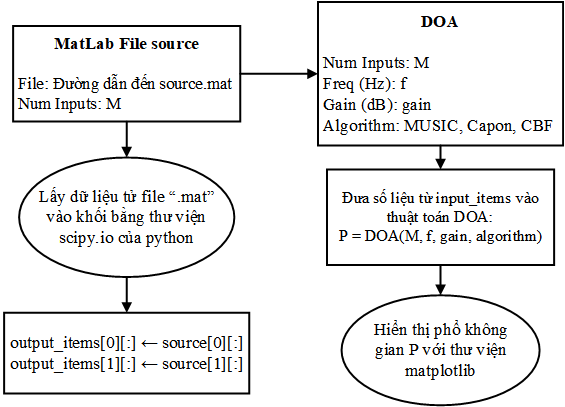
\includegraphics[width=0.9\linewidth]{figures/simulation.png}
	\caption{Sơ đồ làm việc DOA với dữ liệu mô phỏng Matlab}
	\label{fig:simulation}
\end{figure}

\subsection{Kết quả thực thi và đánh giá}

Lập trình khối theo sơ đồ khối \ref{fig:simulation}, cài đặt và tích hợp chúng vào GNU Radio, liên kết 2 khối, kết quả như hình \ref{fig:simulation1}.

\begin{figure} [!hb]
	\centering
	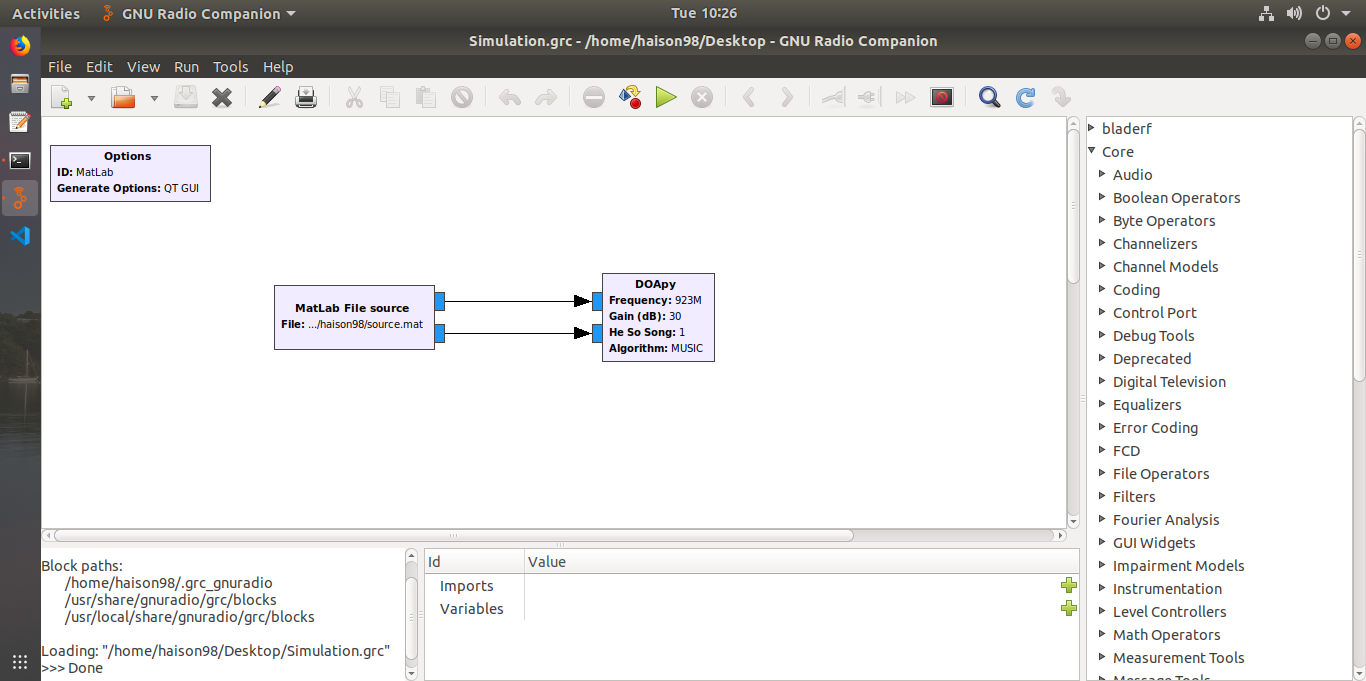
\includegraphics[width=1\linewidth]{figures/simulation1.png}
	\caption{Flow-graph ước lượng DOA với dữ liệu mô phỏng Matlab trên GNU Radio}
	\label{fig:simulation1}
\end{figure}

Nhập thông số đầu vào cho 2 khối và chạy chương trình. Kết quả thu được như hình \ref{fig:simulation2}.

\begin{figure}[h]
%\hfill
\subfigure[Kết quả của GNU Radio]{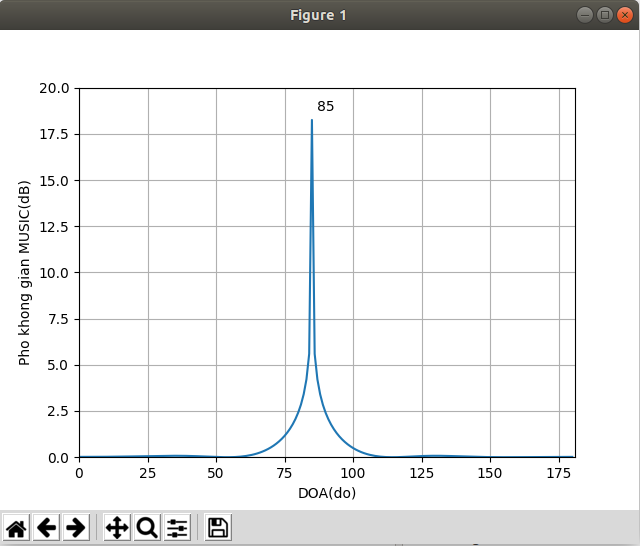
\includegraphics[width=0.49\linewidth]{figures/simulation3.png}}
\hfill
\subfigure[Kết quả của Matlab]{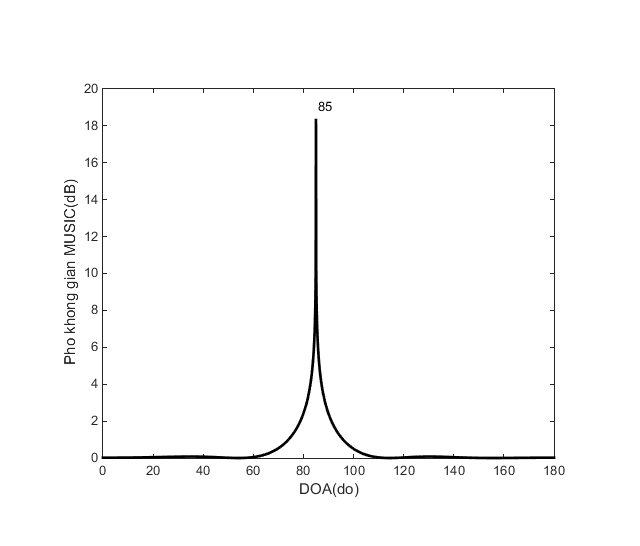
\includegraphics[width=0.49\linewidth]{figures/simulation4.png}}
\hfill
\caption{Kết quả ước lượng DOA với dữ liệu mô phỏng Matlab}
\label{fig:simulation2}
\end{figure}

Có thể thấy, với các thông số đầu vào lý tưởng, thuật toán chạy ổn định và đưa ra ước lượng DOA chính xác với mô phỏng trên Matlab trước đó. Đây là tiền đề để thực hiện hệ thống trên dữ liệu thực từ SDR.

\section{Thực thi hệ thống trên SDR với dữ liệu thực}

Sau khi đã mô phỏng thành công thuật toán trên GNU Radio với dữ liệu từ Matlab, bước tiếp theo là đưa BladeRF vào hệ thống để lấy dữ liệu thực tế. Tất nhiên từ việc sử dụng mô phỏng sang phần cứng sẽ gặp nhiều khó khăn hơn, tất cả sẽ được trình bày dưới đây.

\subsection{Đồng bộ hệ SDR}

Không giống như dữ liệu mô phỏng đã được căn chỉnh hoàn toàn, dữ liệu thực tế từ hệ SDR sẽ gặp các vấn đề cần phải được xử lý: xung đồng hồ khác nhau; vấn đề $\textrm{DC}_\textrm{offset}$ và cân bằng mẫu IQ cho các từng thiết bị SDR;  việc truyền/nhận dữ liệu từ GNU Radio trên máy tính đến các SDR qua cổng USB thường không được thực hiện đồng thời, dẫn đến hiện tượng các các SDR bắt đầu chạy và gửi mẫu về ở các thời gian khác nhau, gây ra trễ mẫu ($\textrm{sample}_{\textrm{offset}}$) trên dữ liệu mảng thu; sai số trong thời gian lấy mẫu (\textrm{time sampling}); độ lệch pha giữa 2 tín hiệu ($\textrm{phase}_{\textrm{offset}}$) ở trạng thái ban đầu; cùng với vấn đề sai số ($f_{\textrm{offset}}$) trong tần số thu của từng SDR. Khi hiệu chỉnh hoàn tất, hệ SDR được đồng bộ thì mới sử dụng được dữ liệu của chúng cho thuật toán DOA để ước lượng phương tới.

\begin{itemize}
	\item \textbf{Đồng bộ xung đồng hồ giữa các thiết bị SDR mảng thu}
\end{itemize}

Việc đầu tiên cần làm với một hệ sử dụng nhiều SDR, hay các hệ truyền thống khác, đó là phải chia được xung đồng hồ chủ trên một thiết bị master, chia cho các thiết bị còn lại, đảm bảo chắc chắn rằng chúng chạy trên cùng 1 xung đồng hồ. Với BladeRF, điều này đã được nhà sản xuất tích hợp sẵn, với cổng SMB (System Management Bus) là chân J62 trên mạch hay \textit{EXT CLK} trong hình \ref{fig:structbladeRF}. Thông thường, với thiết lập trong \textit{bladerf-cli} (client điều khiển của BladeRF) cổng SMB cho phép xuất xung tham chiếu (REF CLK) ở tần số 38.4 MHz, điện áp 3.6 V, chỉ đủ để chia cho 1 BladeRF khác, do khi hao hụt công suất mỗi khi kết nối thêm BladeRF, yêu cầu mức điện áp tối thiểu của REF CLK ở đầu vào là 3.3 V. Vì vậy để sử dụng được nhiều BladeRF trong mảng thu hơn, bắt buộc phải cần thêm 1 bộ chia xung có bù công suất, có nhiều lựa chọn như Silicon Labs SI5338 Clock Generator Evaluation Board, sử dụng cùng loại IC SI5338 như trên BladeRF cho phép chia xung tối đa đến 8 thiết bị khác.

\begin{figure} [!h]
	\centering
	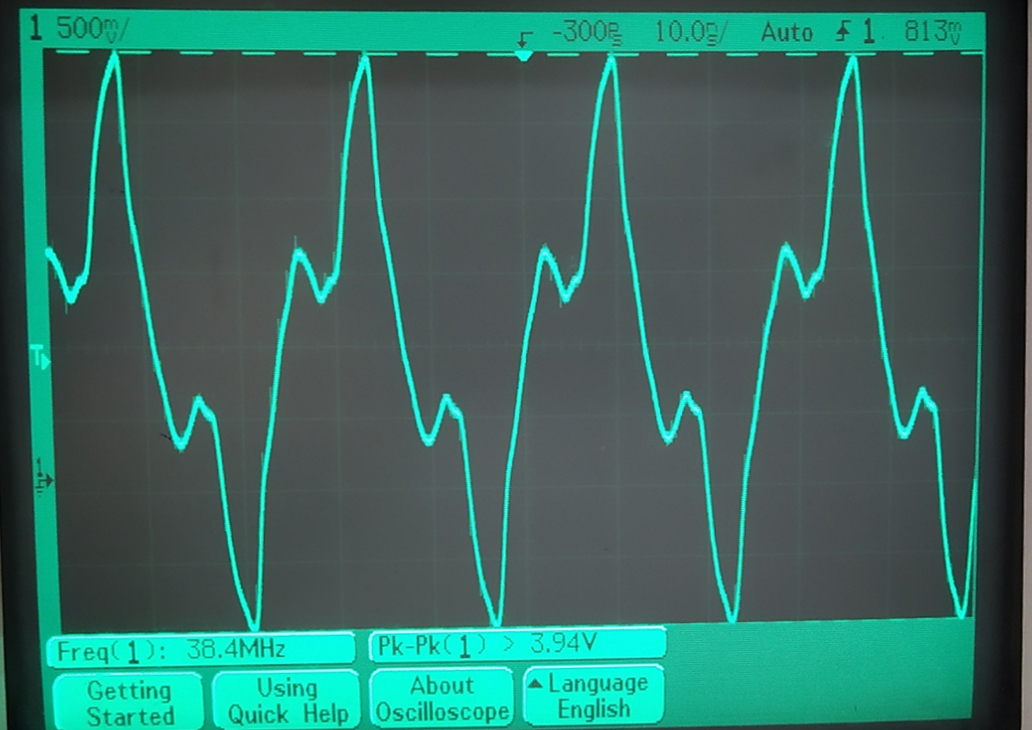
\includegraphics[width=0.75\linewidth]{figures/clk.jpg}
	\caption{Xung đồng hồ tham chiều đầu ra của BladeRF}
	\label{fig:clk}
\end{figure}

%Khi các BladeRF đã kết nối cổng SMB với nhau thông qua bộ chia, thực hiện thiết lập 1 BladeRF làm master (SMB Output) và 3 BladeRF còn lại nhận xung tham chiếu đó (SMB Input) trong client. Tuy nhiên, chỉ chia xung đồng hồ lại chưa đủ để đồng bộ 4 BladeRF, việc truyền/nhận dữ liệu từ GNU Radio trên máy tính đến các BladeRF qua cổng USB thường không được thực hiện đồng thời, dẫn đến hiện tượng các các BladeRF bắt đầu chạy và gửi mẫu về ở các thời gian khác nhau, gây ra hiện tượng trễ mẫu $\textrm{sample}_{\textrm{offset}}$ trên dữ liệu mảng thu. Cùng với vấn đề do sai số ($f_{\textrm{offset}}$) gây ra sự sai khác từ 1-2 Hz trong tần số thu của từng BladeRF (/todo PLL khác nhau). Dưới đây là các phương pháp hiệu chỉnh để hệ thu đồng bộ:

\begin{itemize}
	\item \textbf{Hiệu chỉnh $\textbf{DC}_{\textbf{offset}}$ và cân bằng  mẫu IQ}
\end{itemize}

Các sai số này đã được nhà sản xuất tính đến và tích hợp sẵn việc hiệu chỉnh trong thư viện của BladeRF. Chi tiết có tại \cite{Dccali}.

\begin{itemize}
	\item \textbf{Hiệu chỉnh $\textrm{sample}_{\textbf{offset}}$}
\end{itemize} 

Để hiệu chỉnh mẫu từ SDR, đã có nhiều dự án được thực hiện với nhiều phương pháp khác nhau với các phương pháp cả bằng phần cứng và phần mềm. Các phương pháp sử dụng thêm phần cứng sẽ đảm bảo tính chính xác phù hợp với những hệ thống nhúng thời gian thực thực hiện chức năng chuyên biệt, hay tín hiệu thu có tính tương quan cao khó xác định bằng các thuật toán trên phần mềm. Ngược lại việc đồng bộ mẫu sử dụng phần mềm lại có tính linh hoạt cao, có thể đồng bộ lượng mẫu đầu vào lớn (chục triệu mẫu), tuy nhiên bị giới hạn độ chính xác bởi môi trường truyền.

\textendash\hspace{0.1cm} Phương pháp sử dụng thêm phần cứng Noise Source Card và tương quan chéo của nhiễu Gauss \cite{kerberos} trên miền thời gian. Ý tưởng là sử dụng giao tiếp I2C để chuyển đổi giữa đầu vào cao tần từ anten và đầu vào từ Noise Source Card. Khi hệ thống bắt đầu hoạt động, các SDR lấy mẫu từ Noise Source Card và thực hiện tính tương quan chéo giữa các SDR. Kết quả tương quan chéo của 2 SDR với nhiễu Gauss, như hình \ref{fig:xcorr}. Nếu đỉnh của phổ tương quan chéo không có vị trí $\mathrm{arg max = 0}$, biểu hiện 2 SDR đang thu mẫu có độ trễ với nhau, vị trí đỉnh của phổ cũng thể hiện chinh xác số mẫu trễ. Vì vậy tiến hành lấy mẫu trễ trên SDR nhanh hơn 1 lượng mẫu bằng vị trí đỉnh đỉnh của phổ tương quan chéo $\mathrm{arg max}$.
\begin{equation}
\begin{split}
\mathbf{x}(t) &  =\textrm{Tín hiệu cơ sở}\\
\cos(\omega t) &=\textrm{Sóng mang}\\
\mathbf{x}_1(t) &=\mathbf{x}(t)\cos(\omega t)\\
\mathbf{x}_2(t) &=\mathbf{x}(t - \tau)\cos(\omega (t - \tau)) \\
\textrm{xcorr}(T) &=\sum_{t = -\infty}^{+\infty} \mathbf{x}_{1} (t) \mathbf{x}_{2} (t + T) \\
\tau &=\textrm{argmax}\textrm{(xcorr}(T)) 
\end{split}
\end{equation}

\begin{figure} [!h]
	\centering
	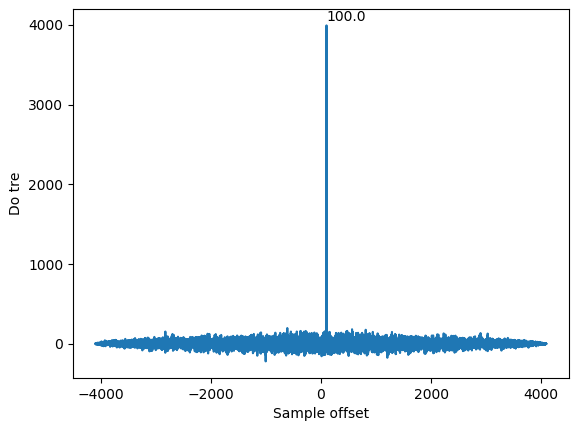
\includegraphics[width=0.9\linewidth]{figures/xcorr.png}
	\caption{Tương quan chéo của 2 nhiễu Gauss}
	\label{fig:xcorr}
\end{figure}

%\begin{figure} [!h]
%	\centering
%	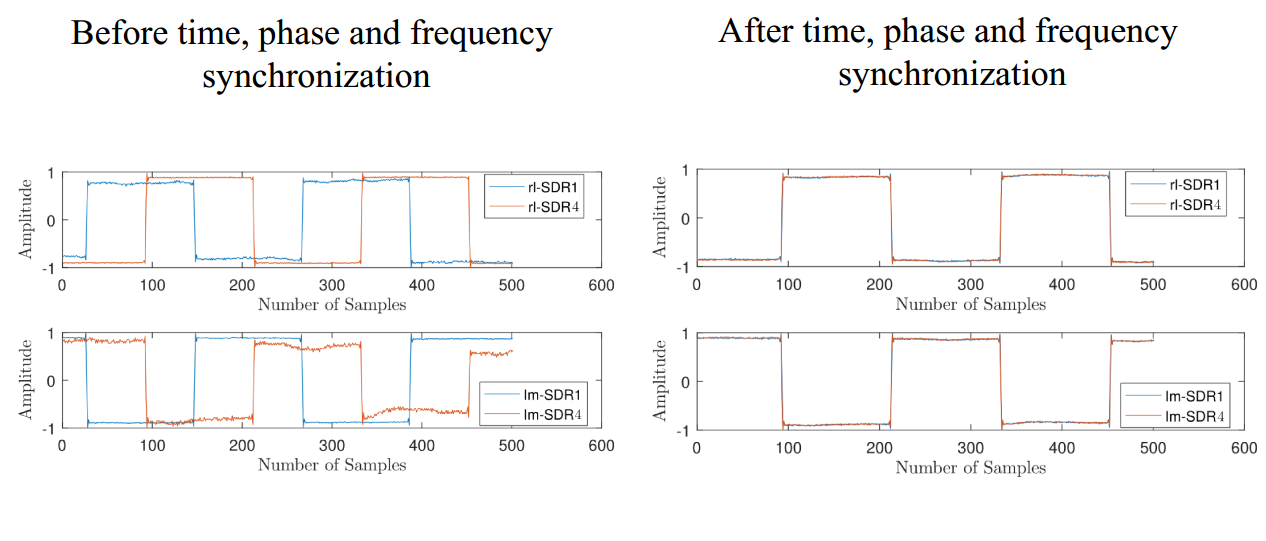
\includegraphics[width=1\linewidth]{figures/sync.png}
%	\caption{Đồng bộ hệ SDR}
%	\label{fig:sync}
%\end{figure}

\textendash\hspace{0.1cm} Phương pháp tiếp theo, sử dụng 1 tín hiệu tham chiếu ở tần số cố định (FM, DVB-T, GSM, ...) được thực hiện trong dự án Multi-RTL \cite{multi-rtl}. Trong dự án kênh BCCH của GSM được sử dụng như tín hiệu tham chiếu để đồng bộ các SDR khác nhau. Đây là phương pháp có tính ứng dụng cao, phù hợp với những dự án khi các thiết bị SDR ở khoảng cách xa nhau (ví dụ như TDOA \cite{SDR}, hay giao thoa kế trong kính thiên văn vô tuyến, ...).

\textendash\hspace{0.1cm} Hai phương pháp trên được sử dụng cho các thiết bị SDR giá rẻ là RTL-SDR, với những thiết bị cao cấp hơn như BladeRF hay USRP, nhà sản xuất đã tích hợp sẵn tính năng MIMO cho phép phát/thu mẫu đồng bộ giữa nhiều thiết bị SDR. Cơ chế là sử dụng thêm 1 xung nhịp nữa làm xung lấy mẫu, với 1 BladeRF làm master và các BladeRF còn lại là slave.

\textendash\hspace{0.1cm}Cũng sử dụng tính tương quan của tín hiệu để tìm độ trễ, tuy nhiên thay vì tính toán ngay trên miền thời gian, việc chuyển sang miền tần số sẽ giúp giảm đáng kể lượng tính toán cần thiết. Sử dụng các phép biến đổi  FFT, IFFT để tính toán trễ giữa hai tín hiệu \cite{Nentwig2016}. Áp dụng trên GNU Radio, với các khối có sẵn FFT, IFFT, Multipy conj, dữ liệu đầu vào là tín hiệu truyền hình chuẩn DVT-T2 được chia thành 2 nguồn, nguồn đầu tiên bị trễ 1000 mẫu so với nguồn thứ 2, lưu đồ tương ứng trên GNU Radio như hình \ref{fig:fft} và kết quả đầu ra biểu diễn qua QT GUI trên hình \ref{fig:dvb-t2} với vị trí đỉnh phổ đúng bằng số lượng trễ mô phỏng.
\begin{equation}
\begin{split}
\mathbf{x}_1(t) &\Leftrightarrow \mathbf{x}_1(f)\\
\mathbf{x}_2(t) &\Leftrightarrow \mathbf{x}_2(f)\\
\textrm{xcorr}(T) &\Leftrightarrow \textrm{xcorr}(f)\\
\textrm{xcorr}(f) &= \mathbf{x}_1(f) \times \mathbf{x}_2(f)^{*}
\end{split}
\end{equation}

%Kết quả thu được, đỉnh của đầu ra IFFT là số mẫu trễ được giả lập từ trước. (/replace lại ảnh với dữ liệu thật)

\begin{figure}[!h]
%\hfill
\centering
\subfigure[Flow-graph mô phỏng ước lượng độ trễ giữa các đầu vào]{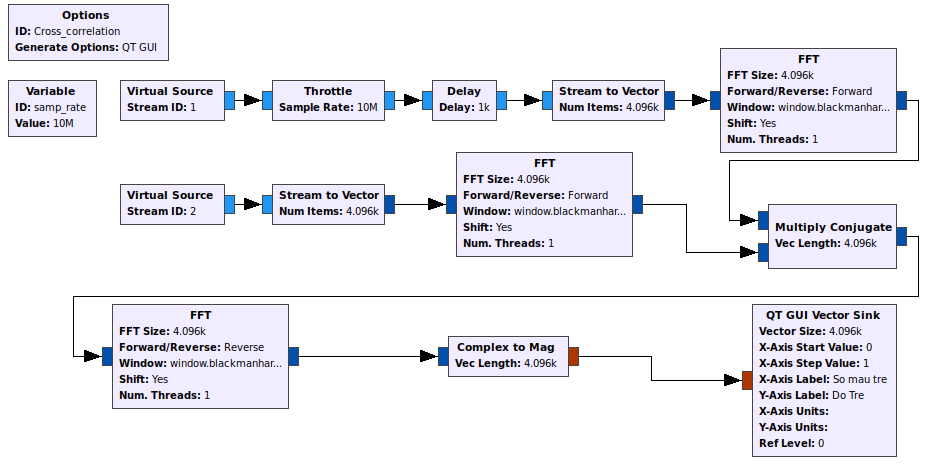
\includegraphics[width=0.9\linewidth]{figures/fft.png}\label{fig:fft}}
\hfill
\subfigure[Phổ tương quan chéo]{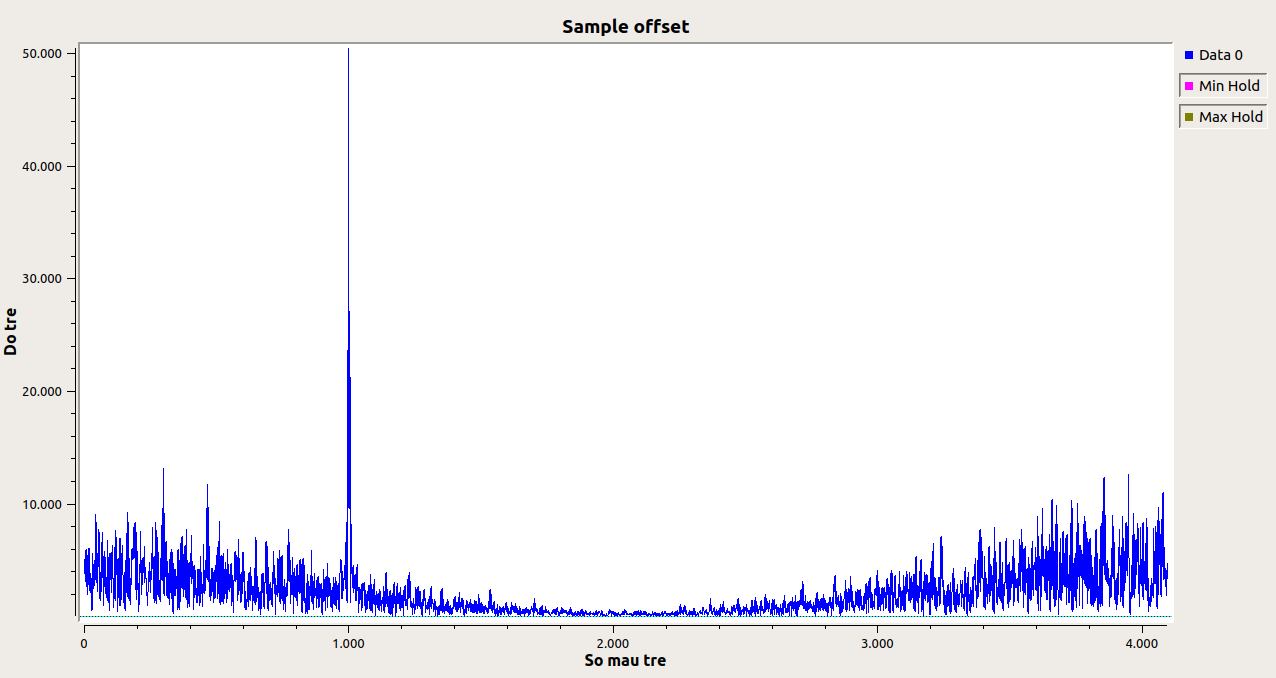
\includegraphics[width=0.9\linewidth]{figures/dvb-t2.png}\label{fig:dvb-t2}}
\hfill
\caption{Xác định độ trễ mẫu trên GNU Radio}
\end{figure}

%\begin{figure} [!h]
%	\centering
%	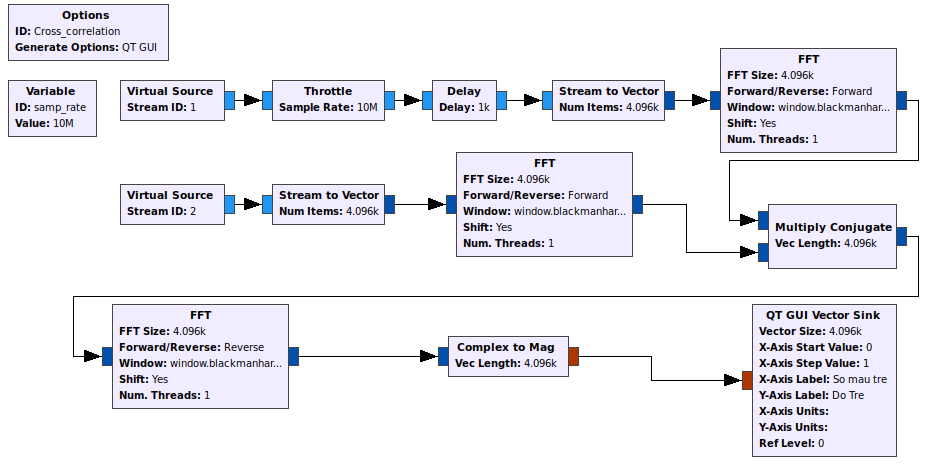
\includegraphics[width=1\linewidth]{figures/fft.png}
%	\caption{Flow-graph mô phỏng ước lượng độ trễ giữa các đầu vào}
%	\label{fig:fft}
%\end{figure}
%\begin{figure} [!h]
%	\centering
%	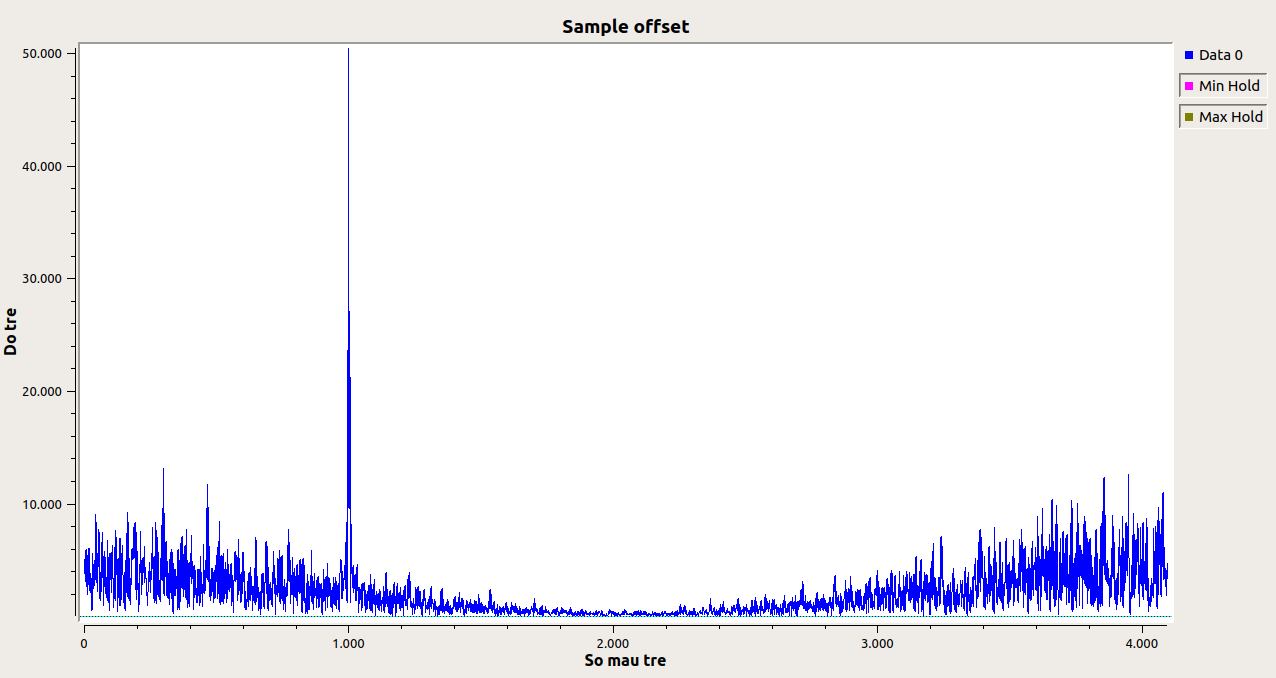
\includegraphics[width=1\linewidth]{figures/dvb-t2.png}
%	\caption{Số mẫu trễ của 2 tín hiệu đầu vào}
%	\label{fig:dvbt2}
%\end{figure}

Sau khi đã có được số mẫu trễ, sử dụng khối Delay, trễ mẫu của khối nguồn đang chạy nhanh đi một lượng $\textrm{argmax(xcorr( f ))}$.  Folow-graph \ref{fig:fft} được viết gọn vào 1 khối duy nhất Sample Offset để tiện cho việc xử lý, $\textrm{sample}_\textrm{offset}$ được lưu vào 1 biến và phản hồi lại về đầu vào để  căn chỉnh dữ liệu khớp với nhau về mặt thời gian sẵn sàng cho các  khối xử lý tiếp theo trong GNU Radio.

\begin{figure}[!h]
%\hfill
\subfigure[Ước lượng $\textrm{sample}_\textrm{offset}$ ]{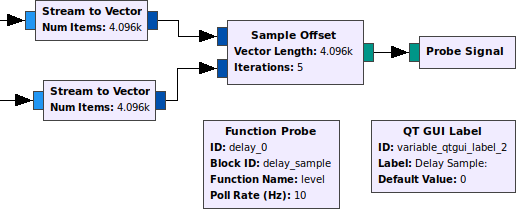
\includegraphics[width=0.6\linewidth]{figures/sample_offset.png}}
\hfill
\subfigure[Phản hồi  $\textrm{sample}_\textrm{offset}$]{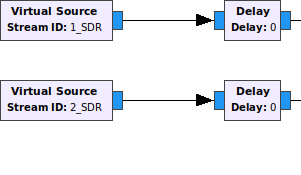
\includegraphics[width=0.35\linewidth]{figures/sample_offset_fb.png}}
\hfill
\caption{Ước lượng và phản hồi hiệu chỉnh $\textrm{sample}_\textrm{offset}$}
\label{fig:sample_offset}
\end{figure}

Nhược điểm của phương pháp này là nếu độ trễ mẫu quá lớn, thông thường lớn hơn 1/2 số mẫu đầu vào khối FFT thì không thể tìm được độ trễ của các nguồn. Vì vậy, số lượng phần tử được đưa vào FFT có thể nâng lên đến hàng trăm nghìn phần tử để chắc chắn rằng thu được độ trễ khớp, nhưng để giảm thiểu tính toán, chỉ cần thực hiện hiệu chỉnh $\textrm{sample}_\textrm{offset}$ khoảng 5 lần đầu tiên và lưu giá trị trễ cố định cho toàn bộ thời gian chương trình chạy. Do một khi luồng dữ liệu từ SDR đã vào được GNU Radio, lượng trễ này sẽ giữ ở mức ổn định.

\begin{itemize}
	\item \textbf{Hiệu chỉnh $\textbf{time sampling}$}
\end{itemize} 

Việc hiệu chỉnh thời gian lấy mẫu giữa các SDR, thường chỉ cần thực hiện với các hệ thông không chia sẻ chung xung đồng hồ hệ thống với nhau, hay sử dụng thêm bất kỳ thiết bị phần cứng nào.

Trên BladeRF, cùng với cổng SMB sử dụng cho chức năng MIMO, chân J71 pin 4 cũng được tích hợp chứng năng đồng bộ thời gian lấy mẫu, bằng việc 1 thiết bị master mỗi khi lấy mẫu sẽ gửi đi một xung qua chân J71 pin 4, các thiết bị slave chỉ thực hiện nhận 1 mẫu cho mỗi xung từ thiết bị master. 

TODO: Có thể hiệu chỉnh cho các SDR hoàn toàn không kết nối với nhau trên GNU Radio: Nội sung mẫu và drift sample

\begin{itemize}
	\item \textbf{$\textbf{Hiệu chỉnh } \textbf{f}_{\textbf{offset}}$ và $\textbf{phase}_\textbf{offset}$}
\end{itemize} 

$\textrm{f}_{\textrm{offset}}$ hay chính xác hơn là tần số sóng mang offset CFO (Carrier Frequency Offset), luôn tồn tại khi LO (Local Oscillator) chịu ảnh hưởng bởi nhiễu điện, chênh lệnh nhiệt độ, ... Những độ lệch này có thể tạo ra $\textrm{f}_{\textrm{offset}}$ và $\textrm{phase}_\textrm{offset}$ ngẫu nhiên. Trên các SDR thương mại, các thông số này đã được tính toán, và được bù lại bởi VCTCXO với độ chính xác là thông số PPM (Parts Per Million). Ví dụ như BladeRF được cân chỉnh ở mức 1 PPM ở nhà máy thì $f_{\textrm{offset}}$ tối đa nếu thu tín hiệu DVB-T2 ở tần số 714 MHz tương đương:
\begin{equation}
f_{\mathrm{offset  max}} = \frac{f_c \times PPM}{10^6} = \frac{714 \times 10^6 \times 1}{10^6} = 714 \textrm{Hz}
\end{equation}

714 Hz là khá lớn, để giảm đi sai số này, nhà sản xuất cung cấp công cụ kalibrate-bladeRF \cite{kali}, cho phép người dùng sử dụng tín hiệu từ 1 kênh thuộc trạm cơ sở GSM ở gần để hiệu chỉnh lại VCTCXO xuống mức 0.002381 PPM, tương đương với việc sai số 714 Hz như trên có thể giảm xuống 1.7 Hz, đủ nhỏ để thực hiện các dự án như biến BladeRF thành trạm cơ sở của GSM hay LTE.

Ngoài phương pháp sử dụng phần mềm, BladeRFx115 cung cấp cổng J71 pin 1 để người dùng sử dụng máy phát chuyên dụng tự hiệu chỉnh VCTCXO bằng tín hiệu 1 xung / giây, hoặc 10 MHz ở mức điện áp 1.8 V.

Đối với những SDR giá rẻ như RTL-SDR v3 có thể thực hiện hiệu chỉnh ngay trên GNU Radio. Giả sử tín hiệu cơ sở $s(k)$ với tần số sóng mang offset $f_{0}$ (hoặc $\omega_{0}$), có biểu diễn toán học:
\begin{equation}
	x(k) = s(k)e^{j(2\pi f_{0} k T + \theta)} + n(k) = s(k)e^{j(\omega_0 k T + \theta)} + n(k)
\end{equation}
với $n(k)$ là tín hiệu nhiễu Gauss có trung bình bằng 0, $T$ là chu kỳ một symbol, $\theta$ là pha của sóng mang và $\omega_0$ là tần số góc.

Trên thực tế, việc phục hồi sóng mang đôi khi được định nghĩa như phục hồi pha sóng mang hay phục hồi tần số sóng mạng. Tất cả chúng đều đưa đến kết quả cuối cùng, là cung cấp một hệ đồng bộ ổn định. Điều này được lý giải do mối liên hệ giữa tần số (f), tốc độ góc ($\omega$) và pha ($\theta$):
\begin{equation}
	\omega = \frac{d\theta}{dt} = 2 \pi f
\end{equation}

Do đó, phục hồi pha của tín hiệu bản chất cũng là phục hồi lại tần số của tín hiệu, đây là phương pháp phổ biến để ước lượng $\textrm{f}_{\textrm{offset}}$ do nó không thể được đo đạt trực tiếp như pha. Cách thông thường để tính pha của tín hiệu lấy mẫu IQ là:
\begin{equation}
	\theta = tan^{-1} \left (\frac{Im (x(k))}{Re(x(k))} \right )
\end{equation}
với $Re$ và $Im$ lần lượt là phần thực và ảo của mẫu IQ. Tương tự với các bộ thu khác, độ lệch pha giữa các SDR sẽ được tính ra liên tục, có thể được sử dụng làm thông số để cân chỉnh hệ SDR. Tuy nhiên trên thực tế, khi áp dụng vào GNU Radio, phương pháp đơn giản này lại thường phát sinh sai số ngẫu nhiên chứ không hoàn toàn ổn định như trên lý thuyết. Cũng như vì mục đích là ước lượng phương tới của tín hiệu, một cách hiệu chỉnh khác được trình bày dưới đây.

Hiệu chỉnh $\textrm{phase}_\textrm{offset}$ trên GNU Radio, để đảm bảo pha ban đầu trên các SDR là như nhau, kết nối các SDR chung 1 anten hoặc điện trở, giả sử các điều kiện là lý tưởng, tín hiệu đầu vào của các SDR là giống nhau vì nếu là tín hiệu giống nhau lý tưởng, góc đầu ra của thuật toán DOA sẽ là 90$^{\circ}$. Sau khi hiệu chỉnh được $\textrm{sample}_\textrm{offset}$ và \textrm{time sampling} như ở  phần trước. Tín hiệu thu được sẽ lệch nhau về pha ($\textrm{phase}_\textrm{offset}$), các bước chính để cân chỉnh:
\begin{itemize}
	\item Tính toán ma trận hiệp phương sai $\mathbf{R}_\mathbf{x}$ của các tín hiệu.
	\item Tìm 2 ma trận giá trị riêng ($\mathbf{\Lambda}$) và vector riêng ($\mathbf{E}$) từ ma trận hiệp phương sai.
	\item Ước lượng góc đầu ra, và trả về sự sai khác pha của SDR.
	\item Phản hồi sai khác pha về một khối Multipy Exp (hay $e^{j\theta}$).
	\item Cân chỉnh liên tục đến ngưỡng cân bằng khi phương sai giảm xuống thấp, giữ lại trạng thái cân bằng.
	\item Gắn anten riêng chỗ mỗi SDR thực hiện ước lượng DOA.
\end{itemize}
Tất cả  được gộp thành 2 khối PCA Phase Diff và Hold, lưu đồ của hiệu chỉnh như hình \ref{fig:phasediff}.

\begin{figure} [!ht]
	\centering
	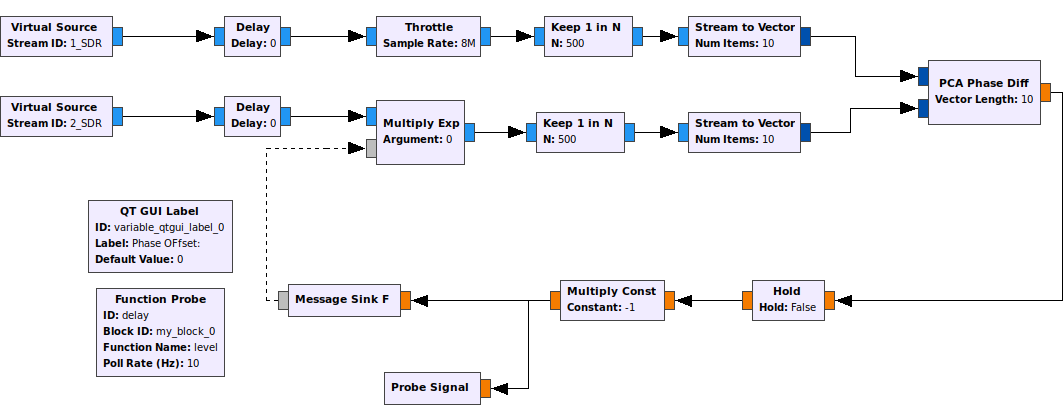
\includegraphics[width=1\linewidth]{figures/phasediff.png}
	\caption{Ước lượng và phản hồi $\textrm{phase}_\textrm{offset}$}
	\label{fig:phasediff}
\end{figure}

\subsection{Mô phỏng dữ liệu thực}

%Dữ liệu thực tế từ các BladeRF được đưa vào GNU Radio qua khối \textbf{gr-osmosdr}, được phát triển dưới dạng mã nguồn mở, sử dụng để đưa dữ liệu từ thư viện của các thiết bị SDR vào GNU Radio, hỗ trợ rất nhiều loại SDR: RTL-SDR, USRP, BladeRF, HackRF, LimeSDR, ... Có sẵn hầu hết các thông số đầu vào của SDR, dễ dàng chỉnh sửa.

Dữ liệu thực tế được dùng cho hệ tìm phương rất da dạng như: tín hiệu FM của các đài phát thanh, tín hiệu chuẩn DVB-T2 của đài truyền hình, GSM hay WiFi,... Dưới đây là folow-graph mô phỏng hai loại tín hiệu phổ biến là FM và DVB-T2.%, 2 loại tín hiệu truyền được ở khoảng các xa do ở tần số dưới 800 MHz, thích hợp cho việc tìm phương.

FM: Điều chế FM trên GNU Radio với file nguồn là file âm thanh nén ở chuẩn WAV (Waveform Audio File Format).

\begin{figure} [!h]
	\centering
	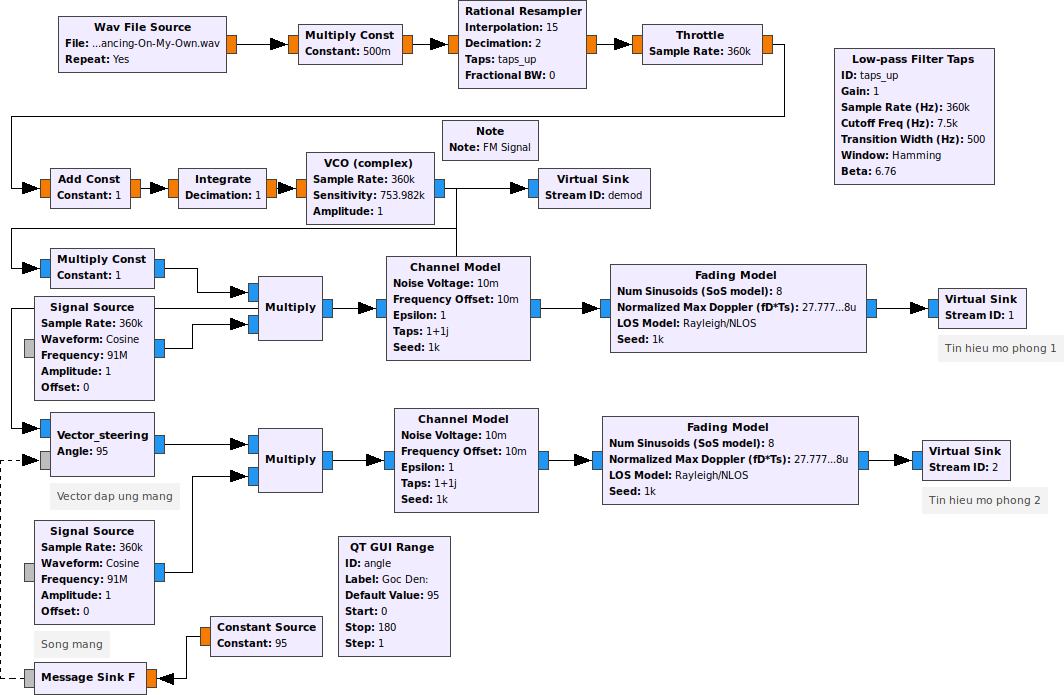
\includegraphics[width=1\linewidth]{figures/fmmod.png}
	\caption{Mô phỏng dữ liệu FM qua kênh truyền}
	\label{fig:fmmod}
\end{figure}

DVB-T2: Điều chế chuẩn DVB-T2 trên GNU Radio với file nguồn là file video nén ở chuẩn TS (Transport Stream).

\begin{figure} [!h]
	\centering
	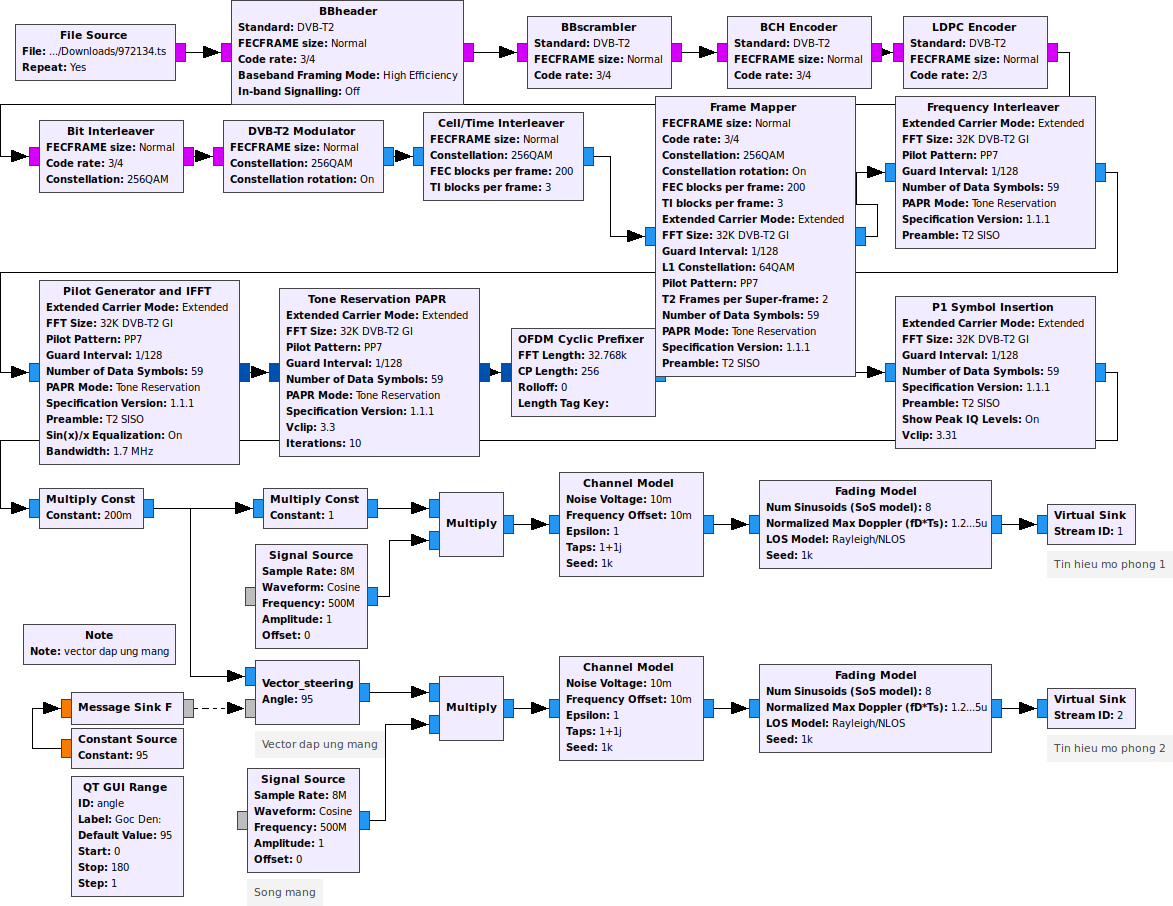
\includegraphics[width=1\linewidth]{figures/dvbt2mod.png}
	\caption{Mô phỏng dữ liệu DVB-T2 qua kênh truyền}
	\label{fig:dvbt2mod}
\end{figure}

Sau khi được điều chế, tín hiệu được chia thành 2 và nhân thêm Vector đáp ứng mảng tương ứng của phần tử SDR 1 và 2 mảng thu, đưa lên tần số cao bằng các khối nguồn cosine tiêu chuẩn 91 MHz và 500 MHz lần lượt ứng với FM và DVB-T2. Tiếp tục đưa qua các khối mô phỏng kênh truyền thực Channel Model (TODO: thông số), và Fading Model (TODO: thông số), đến đây là hoàn tất mô phỏng tín hiệu đến 2 phần tử mảng thu, tiếp theo đưa vào một kênh mô phỏng để thêm các thông số offset của SDR vào tín hiệu.

Tín hiệu của phần tử đầu SDR đầu tiên, được mô phỏng có $\textrm{phase}_\textrm{offset}$ là 45$^{\circ}$, còn SDR thứ 2 được mô phỏng bị trễ 1000 mẫu do phần cứng gây ra.

Mô phỏng việc ước lượng DOA trên GNU Radio: ban đầu 2 SDR chung 1 anten hoặc điện trở, nên tín hiệu chúng thu được sẽ được giả sử là một nhiễu Gauss. Tiến hành đồng bộ hóa $\textrm{sample}_\textrm{offset}$ và $\textrm{phase}_\textrm{offset}$ trên nhiễu Gauss này. Thu được các thông số đồng bộ là số mẫu delay từ khối Sample Offset và sai khác pha từ khối PCA Phase Diff. Giữ nguyên các thông số này, chuyển hệ từ chung 1 anten (Gauss Noise) sang tín hiệu thực được điều chế, ước lượng DOA đầu ra sẽ được hiển thị thời gian thực qua giao diện QT GUI.

TODO: Phân tích kênh truyền

TODO: Hjx có khi em nên đưa vào 1 cái lưu đồ đoạn text trên

\subsection{Sơ đồ khối và mô tả sơ đồ khối}

%\begin{figure} [!h]
%	\centering
%	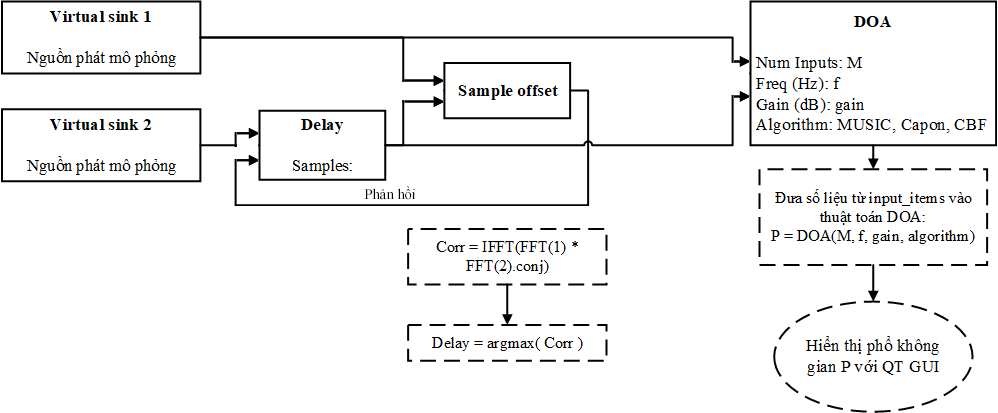
\includegraphics[width=1\linewidth]{figures/SimulationDOA.png}
%	\caption{Sơ đồ làm việc DOA với mô phỏng dữ liệu thực}
%	\label{fig:SimulationDOA}
%\end{figure}

%Tiến hành, bố trí hệ thống DOA với 4 BladeRF làm mảng thu và 1 BladeRF làm nguồn phát tín hiệu như mô tả trên hình \ref{fig:DOAsys}. Tiếp đến là công việc hiệu chỉnh lại hệ thống bằng phần mềm được trình bày ở phần tiếp theo.

%\begin{figure} [!hb]
%	\centering
%	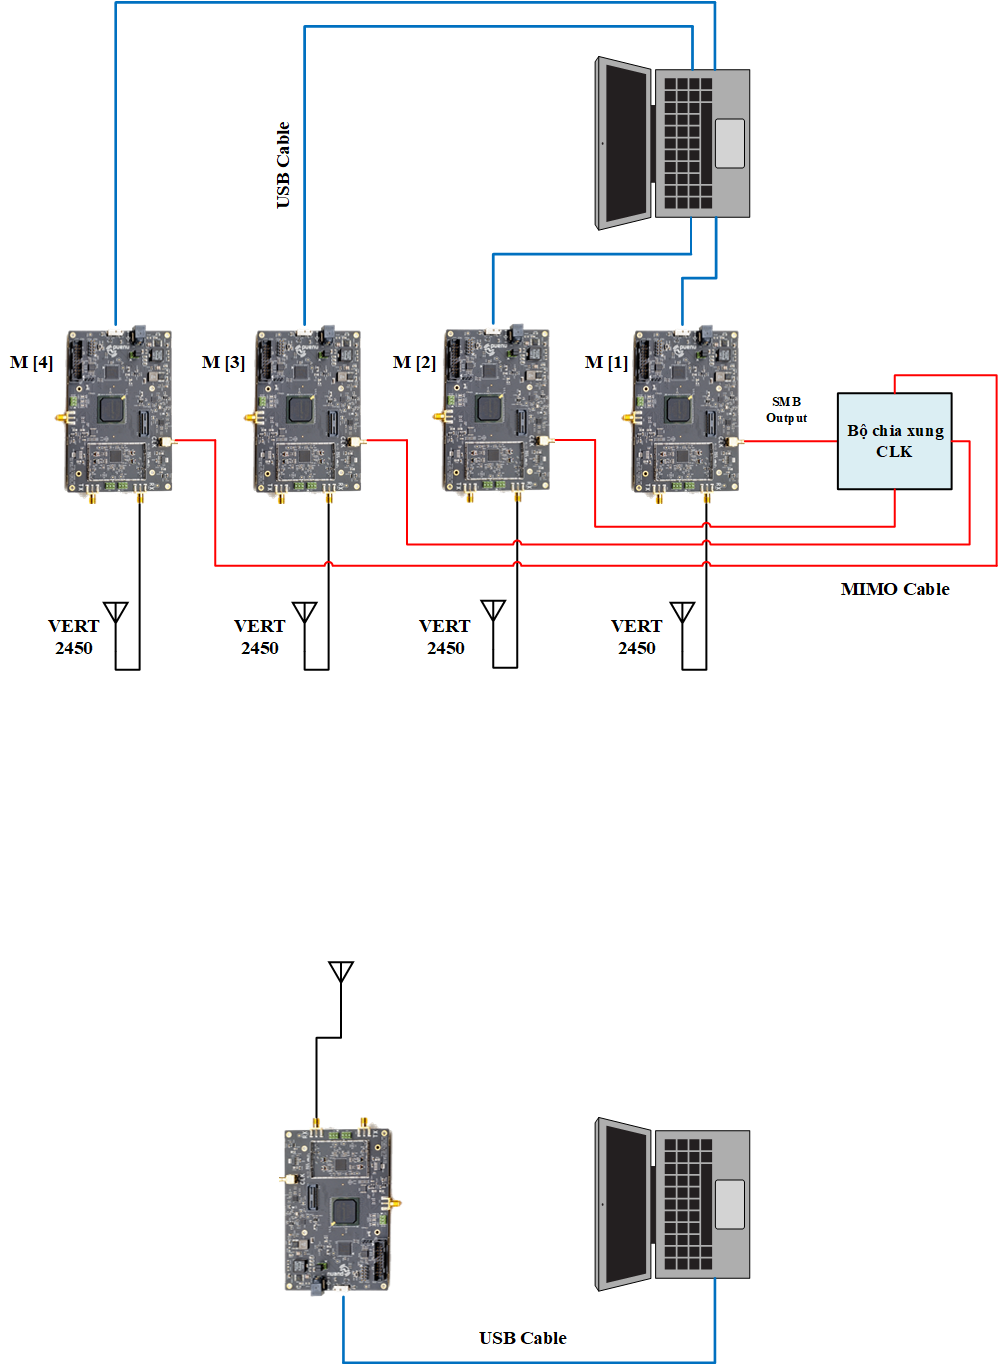
\includegraphics[width=1\linewidth]{figures/DOAsys.png}
%	\caption{Sơ đồ bố trí hệ DOA sử dụng 5 BladeRF}
%	\label{fig:DOAsys}
%\end{figure}

%(/todo anten) Hình ảnh thực tế của hệ DOA sử dụng BladeRF trên hình \ref{fig:DOAsysreal}.
%\begin{figure} [!ht]
%	\centering
%	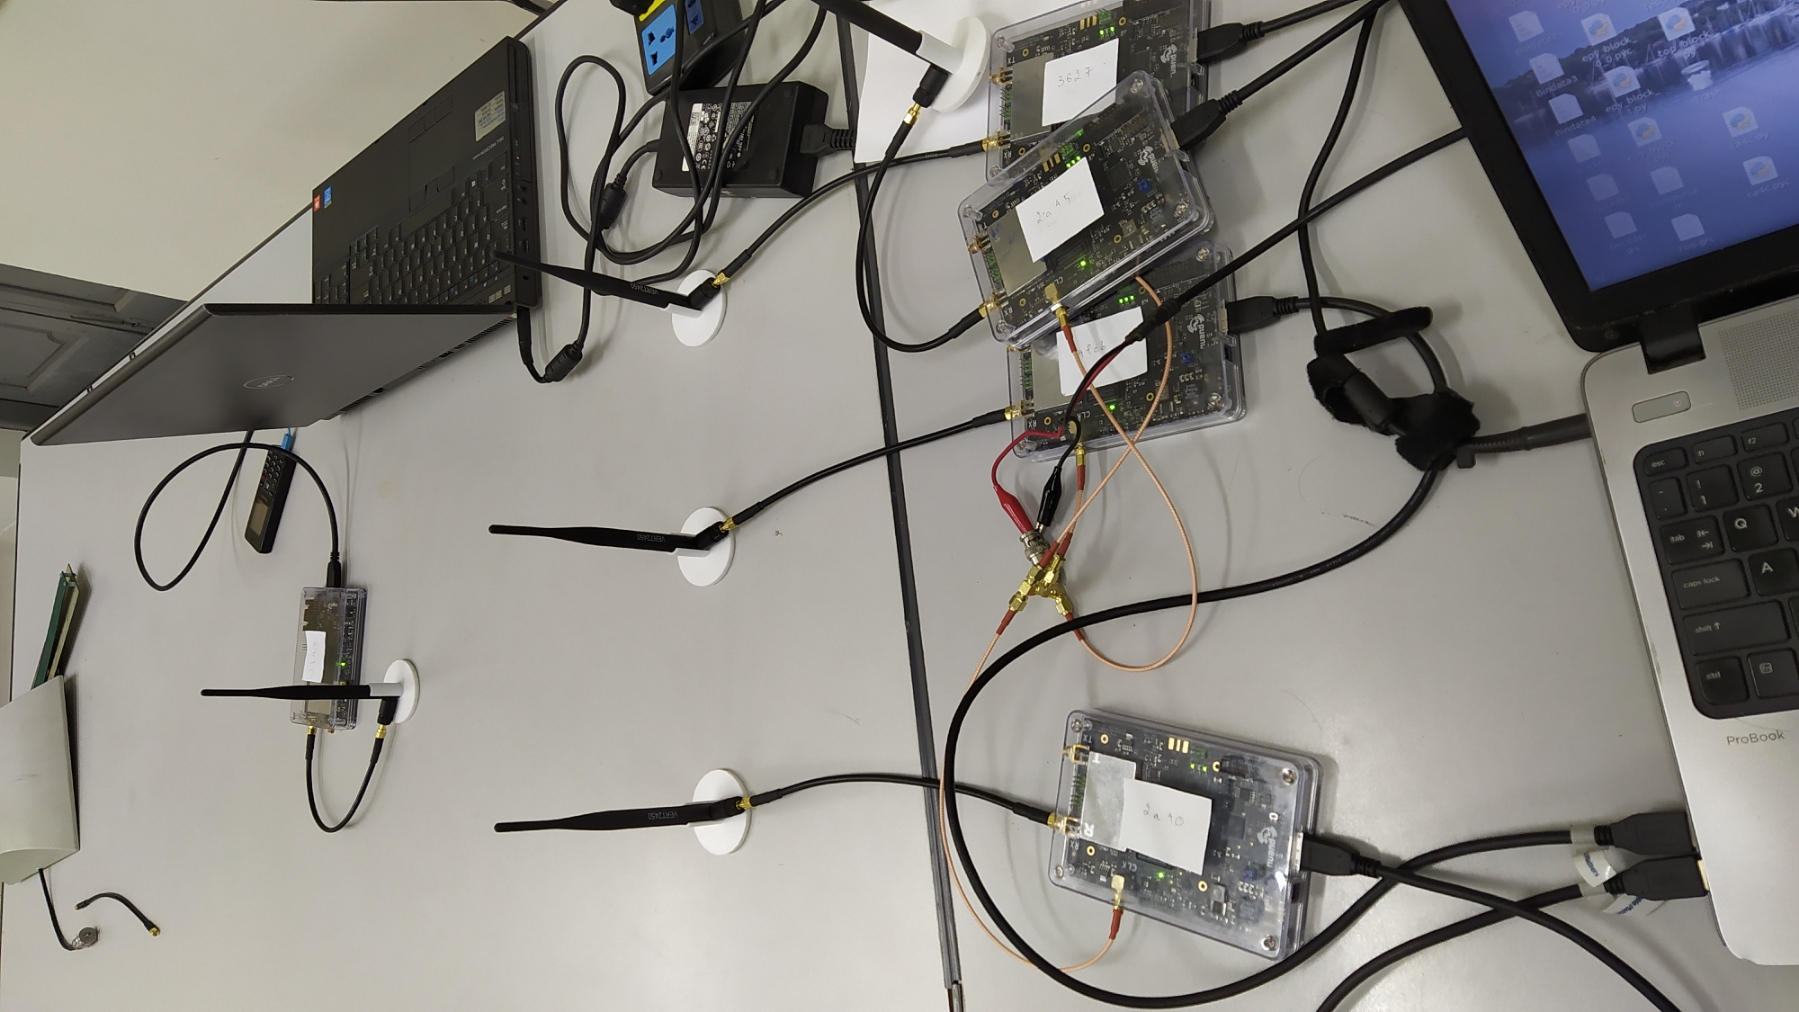
\includegraphics[width=1\linewidth]{figures/DOAsysreal.jpg}
%	\caption{Hệ DOA sử dụng BladeRF}
%	\label{fig:DOAsysreal}
%\end{figure}

Thông số các khối trong hệ DOA:
{\renewcommand\labelitemi{}
\begin{itemize}
	\item $f_{\textrm{FM}} = 91\textrm{MHz}$			\hspace{1.3cm}\% Tần số tín hiệu FM
	\item $f_{\textrm{DVB-T2}} = 500\textrm{MHz}$		\hspace{0.45cm}\% Tần số tín hiệu DVB-T2
	\item $d = 0.5 \times \lambda$		\hspace{1.85cm}\% Khoảng cách giữa các phần tử anten mảng thu (\textbf{ULA})
	%\item $\lambda = c \div f =  m$	\hspace{0.47cm}\% Bước sóng
	\item $M = 2$				\hspace{2.68cm}\% Số phần tử anten của mảng thu
	\item $D = 1$				\hspace{2.77cm}\% Số phần tử nguồn
	%\item $angle = 85 \times (\pi \div 180)$ \% Góc tới của tín hiệu
	\item $gain = 0 dB$			\hspace{1.75cm}\% Hệ số khuếch đại
	%\item $SNR = 15 dB$			\hspace{1.57cm}\% Tỷ lệ tín hiệu tạp âm
	%\item $k = 2 \times \pi \div \lambda$	\hspace{1.56cm}\% Hệ số sóng
	%\item $K = 4096$				\hspace{2.3cm}\% Số mẫu thu thập	
\end{itemize}
\begin{figure} [!ht]
	\centering
	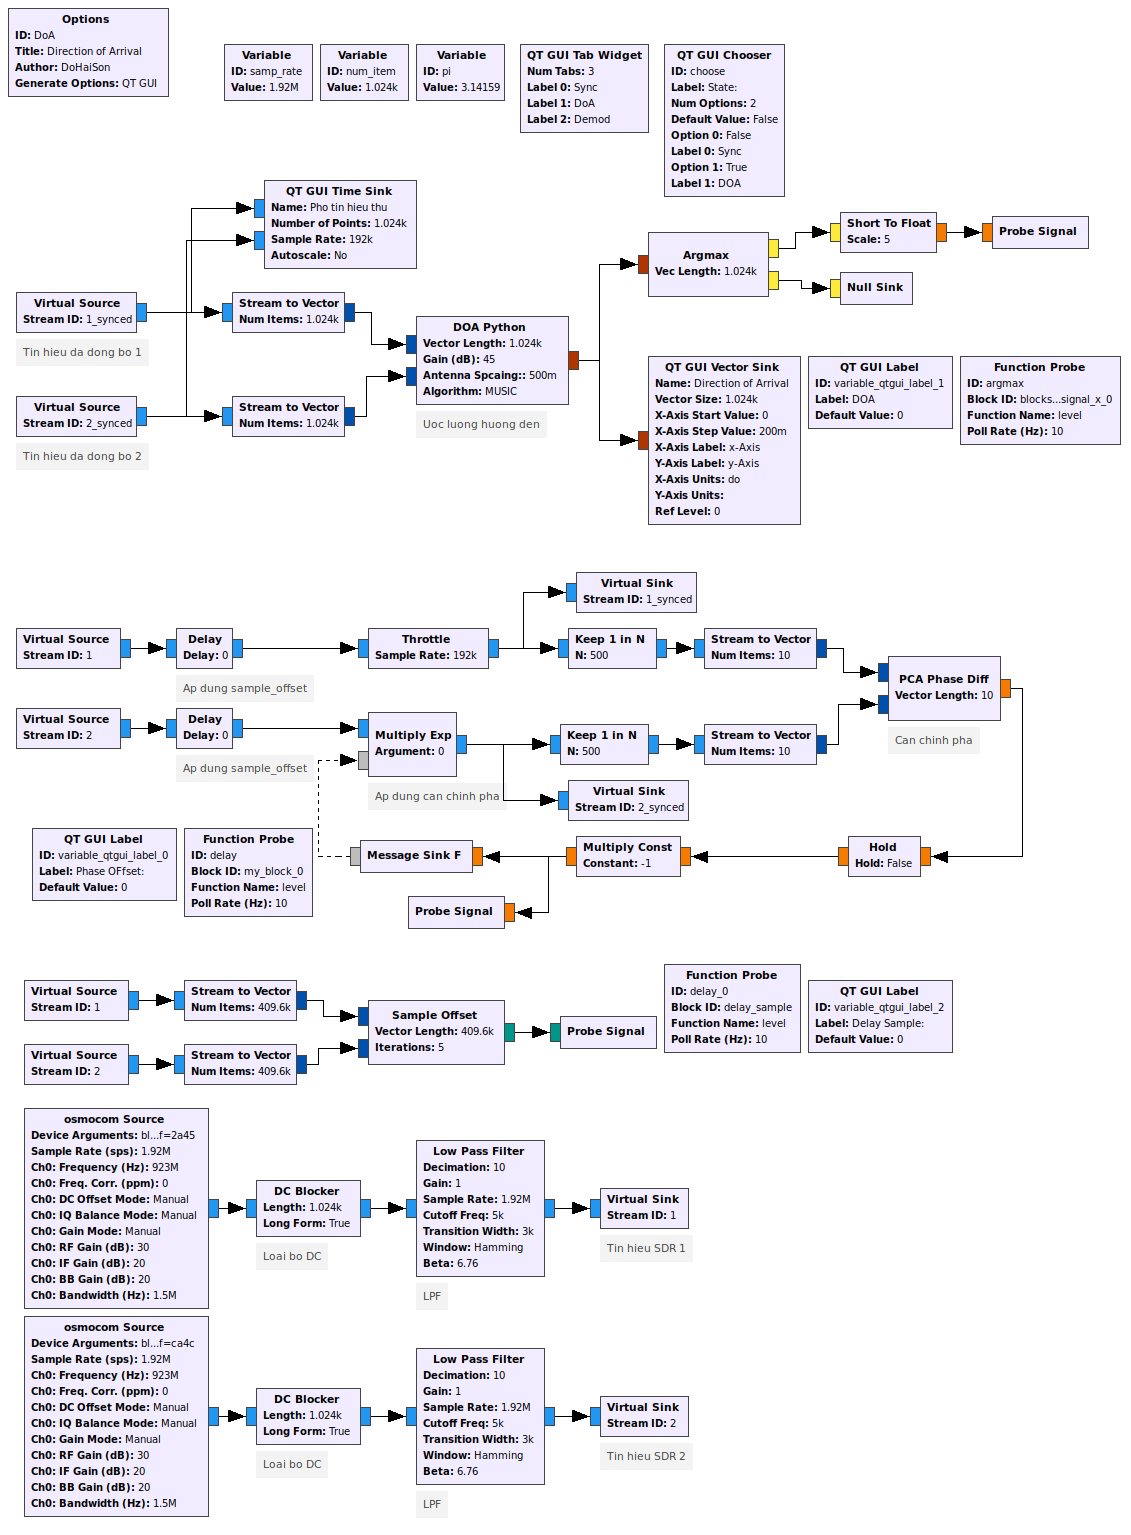
\includegraphics[width=\textwidth,height=\textheight,keepaspectratio]{figures/DoA_FM_grc.png}
	\caption{Flow-graph ước lượng DOA}
	\label{fig:DoA_FM}
\end{figure}

\subsection{Kết quả thực thi và đánh giá}

\begin{table}[!h]
\centering
\begin{tabular}{lcc}
\hline
\rowcolor[HTML]{FFE8E7} 
\multicolumn{1}{c}{\cellcolor[HTML]{FFE8E7}\textbf{Thông số}} & \textbf{Bên phát} & \textbf{Bên thu} \\ \hline
CPU & Intel Core I5-4210M & Intel Core I5-4800MQ \\
RAM & 8 GB & 8 GB \\
Hệ điều hành & Ubuntu 18.04 LTS & Ubuntu 16.04 LTS \\
Phiên bản GNU Radio & 3.7.11 & 3.7.11 \\ \hline
\end{tabular}
\caption{Thông số máy tính}
\label{table:hw}
\end{table}

Kết quả ước lượng DOA mô phỏng với tín hiệu chuẩn DVB-T2 lý tưởng với trường hợp có nhiễu và fading.

\begin{figure}[!h]
%\hfill
\centering
\subfigure[Ước lượng $\textrm{sample}_\textrm{offset}$ và $\textrm{phase}_\textrm{offset}$ ]{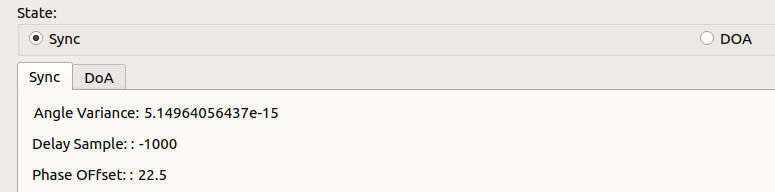
\includegraphics[width=0.75\linewidth]{figures/DOA_DVB-T2_1.png}\label{fig:DOA_DVB-T2_1}}
\hfill
\subfigure[Giữ lại các thông số hiệu chỉnh]{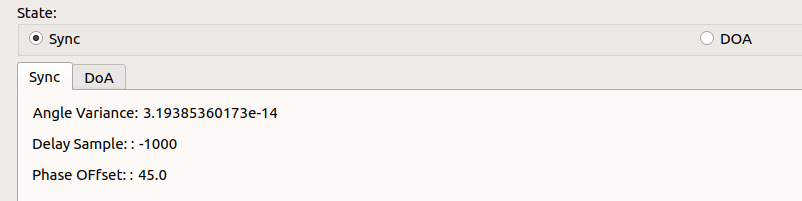
\includegraphics[width=0.75\linewidth]{figures/DOA_DVB-T2_2.png}\label{fig:DOA_DVB-T2_2}}
\hfill
\subfigure[Ước lượng DOA góc đầu vào 95$^{\circ}$]{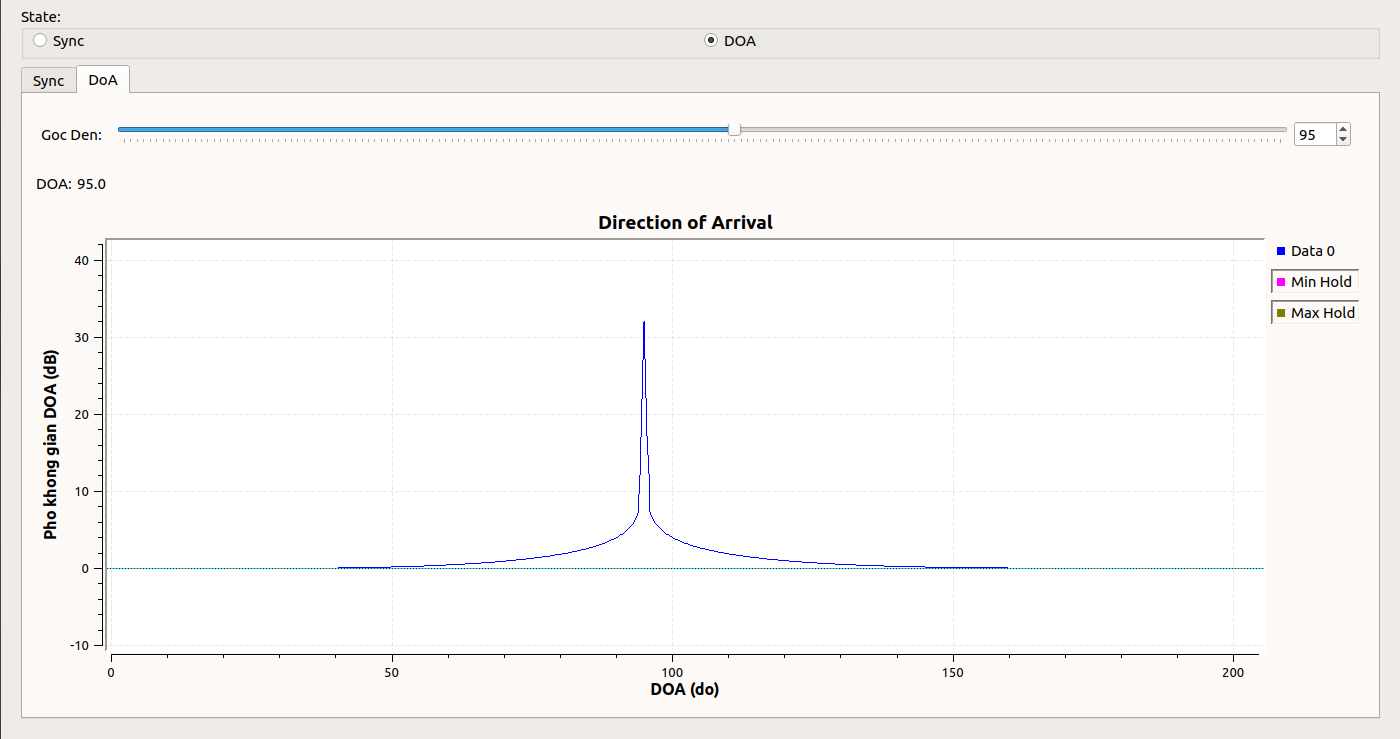
\includegraphics[width=0.85\linewidth]{figures/DOA_DVB-T2_3.png}\label{fig:DOA_DVB-T2_3}}
\hfill
\subfigure[Ước lượng DOA góc đầu vào 149$^{\circ}$]{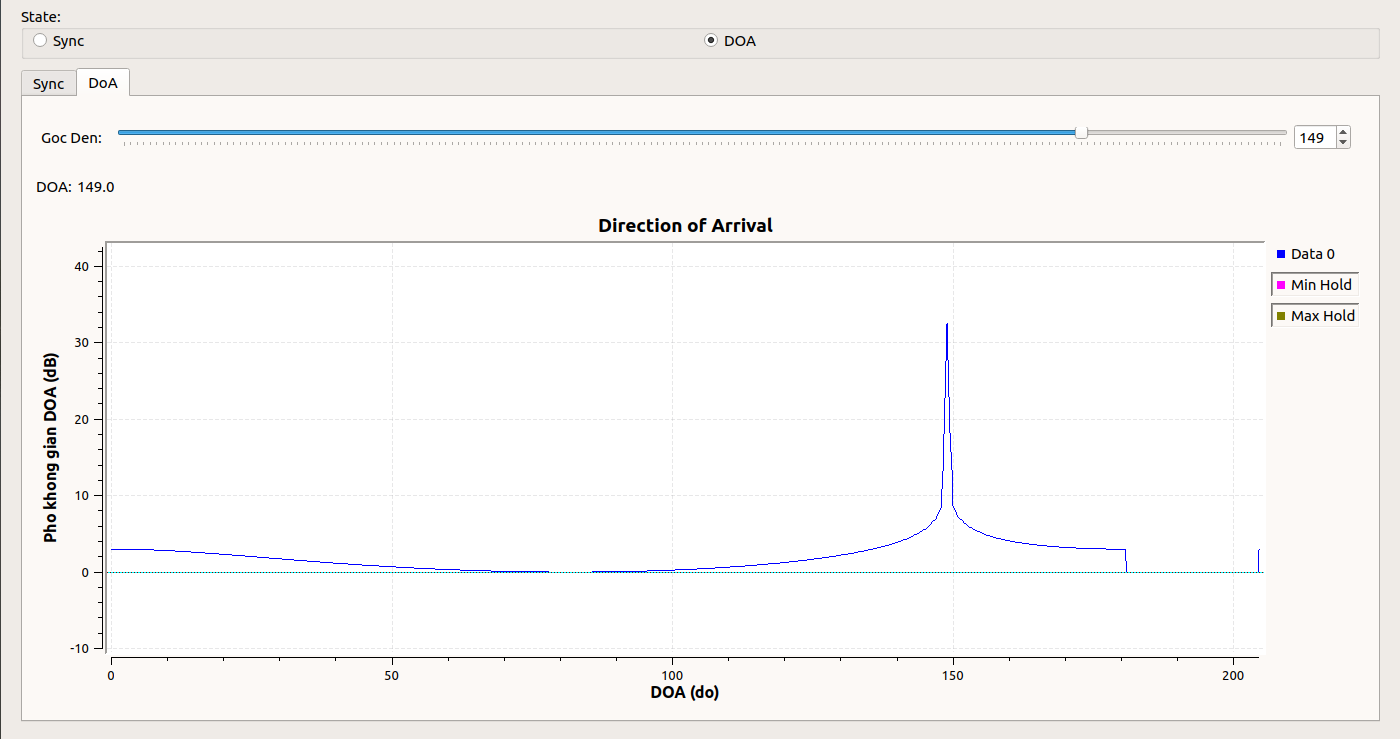
\includegraphics[width=0.85\linewidth]{figures/DOA_DVB-T2_4.png}\label{fig:DOA_DVB-T2_4}}
\hfill
\caption{Uớc lượng DOA với tín hiệu DVB-T2, kênh truyền lý tưởng}
\end{figure}
\begin{figure}[!h]
%\hfill
\centering
\subfigure[Ước lượng $\textrm{sample}_\textrm{offset}$ và $\textrm{phase}_\textrm{offset}$ ]{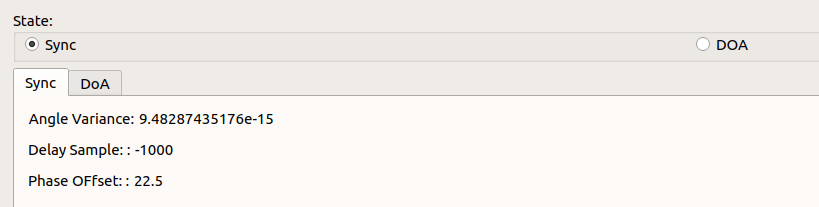
\includegraphics[width=0.75\linewidth]{figures/DOA_DVB-T2_Noise_1.png}\label{fig:DOA_DVB-T2_Noise_1}}
\hfill
\subfigure[Giữ lại các thông số hiệu chỉnh]{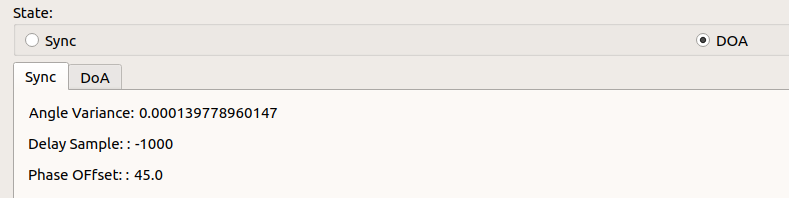
\includegraphics[width=0.75\linewidth]{figures/DOA_DVB-T2_Noise_2.png}\label{fig:DOA_DVB-T2_Noise_2}}
\hfill
\subfigure[Ước lượng DOA góc đầu vào 95$^{\circ}$]{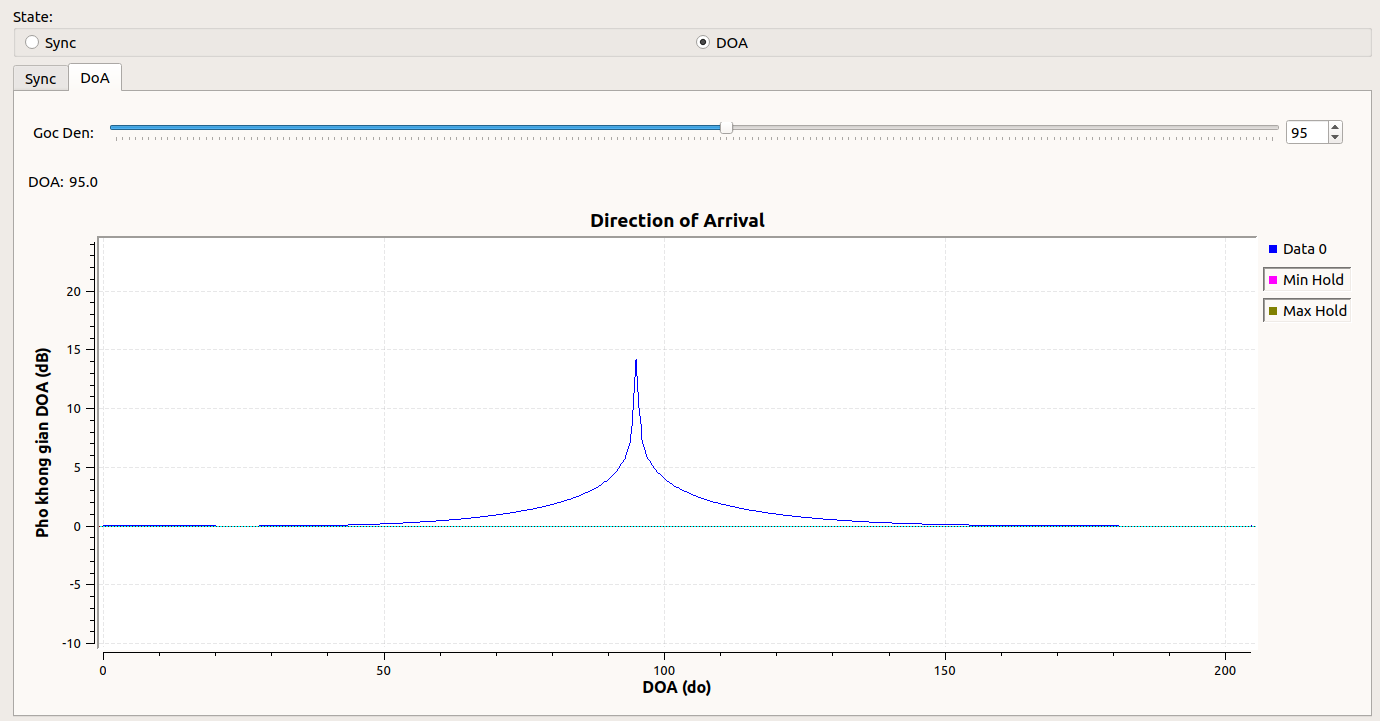
\includegraphics[width=0.85\linewidth]{figures/DOA_DVB-T2_Noise_3.png}\label{fig:DOA_DVB-T2_Noise_3}}
\hfill
\subfigure[Ước lượng DOA góc đầu vào 23$^{\circ}$]{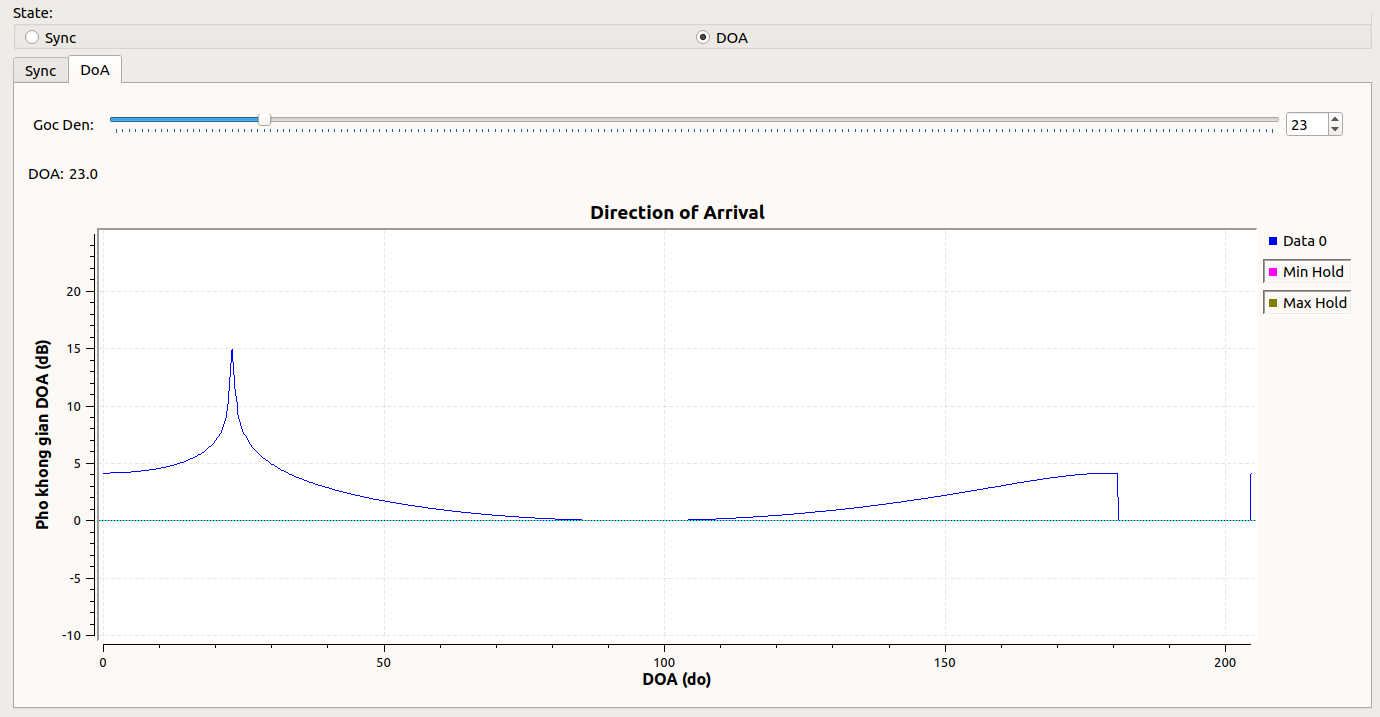
\includegraphics[width=0.85\linewidth]{figures/DOA_DVB-T2_Noise_4.png}\label{fig:DOA_DVB-T2_Noise_4}}
\hfill
\caption{Ước lượng DOA với tín hiệu DVB-T2, kênh truyền nhiễu và fading}
\end{figure}




Đánh giá gì đó @@

\begin{figure} [!h]
	\centering
	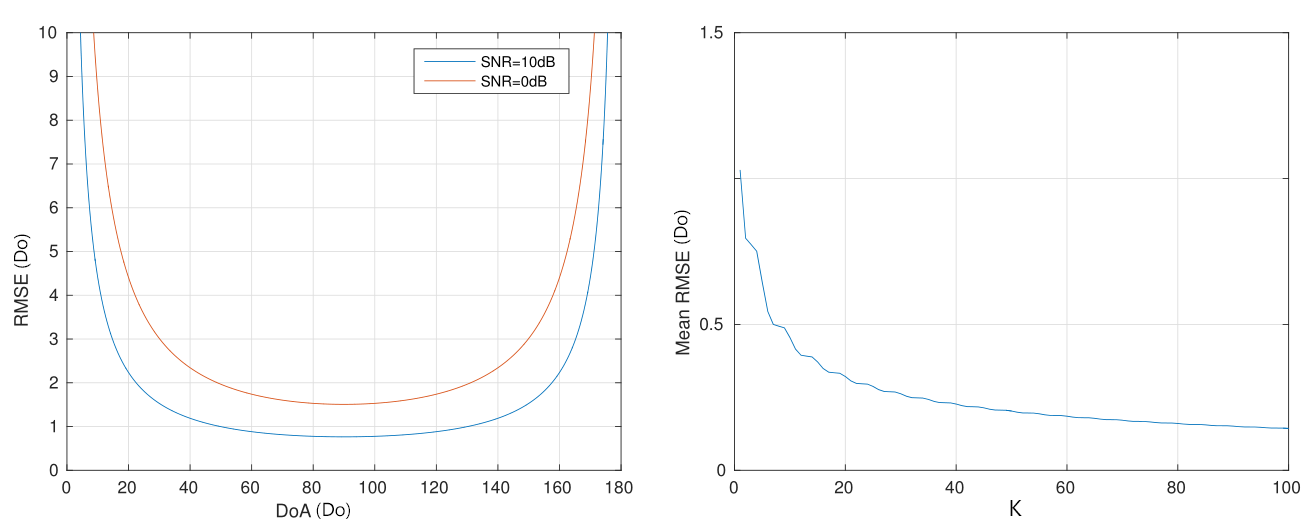
\includegraphics[width=0.7\linewidth]{figures/RMSE.png}
	\caption{Ảnh trên mạng :v}
	\label{fig:RMSE}
\end{figure}